
\chapter*{Introduction}
\addstarredchapter{Introduction}

Appuyer sur le fait que le temps est continu et que l'on veut garder toute l'information pour faire des description super fine temporellement.

\chapter{État de l'art sur la détection de communautés et les réseaux dynamiques}
\minitoc
\label{chap:etat_art}
Dans cette thèse, nous étudions deux axes de recherches liés aux graphes qui sont orthogonaux.
D'une part, il s'agit de la détection de structures dans les graphes et plus particulièrement de communautés.
Un communauté est un sous-ensemble de n\oe uds de manière à ce qu'ils soient fortement connectés.
Il n'existe cependant aucune définition exact et la notion de communauté fortement connectée dépends du contexte et de la méthode.
Malgré cette définition floue, des structures communautaires ont été trouvées dans de nombreux graphes dans plusieurs domaines tel que le réseaux constitué des région du cerveau \cite{DeReus2014}, le réseau de distribution d'eau \cite{DiNardo2015} et un réseau d'interactions d'animaux \cite{Farine2015}.
Ces notions de communautés et les méthodes de détection sont définies dans la section~\ref{sec:intro_communaute}.\\

D'autre part, il a été observé que la modélisation d'un réseau sous la forme d'un graphe peut poser problème notamment quand le réseau change au cours du temps \cite{Holme2015b}.
D'une part, l'information temporelle est complètement perdue lorsque l'on manipule un graphe.
Par conséquent, certaines structures peuvent devenir indétectable.
Imaginons un graphe représentant les alliances politiques dans un pays.
Si toutes les alliances politiques sont agrégées sur une trop grande durée temporelle, alors une personne politique changeant de parti politique sera faussement considérée comme influente car connectée à plusieurs partis alors qu'elle peut ne plus avoir de contact dans son ancien parti.
Ainsi il n'est plus possible d'observer le glissement des alliances politiques dans ce genre de réseau si l'agrégation temporelle est trop importante~\cite{Mucha2010}.

D'autre part, si on prends en compte le temps, alors il est possible de détecter des structure plus fine que dans le cas statique.
Il devient possible de détecter des instant où l'organisation générale change~\cite{Rosvall2010}, de comprendre à quels sont les instant où une personnes est importante~\cite{Magnien2015}, ou bien de détecter des groupes temporelles~\cite{Cazabet2010}.
Face à ces problèmes plusieurs extensions de la théorie des graphes ont été proposées et elles sont résumées dans la section~\ref{sec:intro_extension_temporelle}.

Mais avant de présenter ces deux axes de recherches, nous revenons dans la section~\ref{sec:def_graphe} sur quelques définitions formelles et notation des graphes que nous utilisons dans cette thèse.
\section{Définition dans les graphes}
\label{sec:def_graphe}

Un graphe $G$ est défini par un couple $(V, E)$  où $V$ est une ensemble de n\oe uds et $E$ un ensemble de liens chaque lien est une paire de n\oe uds.
Sauf mention contraire, nous considérons des graphes non-orienté, c'est-à-dire pour toute pair de n\oe uds $u,v \in V$ les liens $(u,v)$ et $(v,u)$ sont équivalents.
Nous considérons également uniquement des liens non-pondérés, c'est-à-dire qu'un lien est soit présent soit absent.
Enfin, nous ne considérons que des graphes simples, c'est-à-dire qu'il n'existe au maximum qu'un seul lien entre deux n\oe uds.
Ceci est en opposition avec les graphes multiples où il peut exister plusieurs liens entre deux n\oe uds.

Par convention, nous définissons $n=|V|$ le nombre de n\oe uds et $m=|E|$ le nombre de liens.
Il est possible de représenter un graphe $G$ par une matrice carré $A$ de taille $n$ où la case $A_{i,j} \ \forall i,j \in \mathbb{N}^+ \leq n$ est égale à $1$ si un lien relie les n\oe uds $i$ et $j$ et $0$ sinon.

\begin{description}
\item[Degré] Le degré d'un n\oe ud $i$, noté $d_i$, est égale au nombre de liens reliés à $i$: $d_u = \sum_{j\leq n} A_{i,j}$.
\item[Densité] La densité, $d(V)$ des n\oe uds d'un graphe est la probabilité que deux n\oe uds soient reliés par un lien: $d(V)=\dfrac{2m}{n(n-1)}$.
\item[Degré moyen] Le degré moyen $\tilde{d}(V)$ diffère de la densité est égale à : $\tilde{d(V)}=\dfrac{2m}{n}$.
\item[Chemin] Une chaine ou chemin entre deux n\oe uds dans un graphe est une suite de liens $((u_1,v_1),...,(u_k,v_k))$ de tel sorte que $v_{i}=u_{i+1} \ \forall i \in [0,k-1]$.
\item[Graphe connexe] Les n\oe uds d'un graphe sont dit connexe s'il existe un chemin entre toute les pairs de n\oe uds.
\item[Composante Connexe] Une composante connexe est un ensemble de n\oe uds $V'\subseteq V$ qui est connexe et maximal, c'est-à-dire qu'il n'est pas possible d'ajouter un n\oe ud dans $V'$ tel que $V'$ soit toujours connexe.
\item[Arbre] Le graphe connexe le moins dense est un arbre et est constitué de $n-1$ liens pour $n$ n\oe uds.
\item[Clique] Le graphe le plus dense est appelé un graphe complet ou un clique et est composé de $\dfrac{n(n-1)}{2}$ pour $n$ n\oe uds.
\item[Sous-graphe] Un graphe $G'=(V',E')$ est un sous-graphe de $G$ si et seulement si $V' \subset V$ et $|E'\cap E| = |E'|$.
\item[Graphe induit] Le graphe induit par un $V' \subset V$ est définit par $V'$ et $E'= \{(u,v) \in E,\ u,v \in V'\}$.  
\end{description}



\subsection{Groupes, partitions et couvertures}
En plus des n\oe uds et des liens, nous manipulons également des ensembles de liens et des ensembles de n\oe uds.
Par convention, soit $X \subset V$ un ensemble de n\oe uds et $Y \subset E$ un ensemble de liens.
Nous listons les notations utilisées dans le tableau~\ref{tab:notation_groupe_noeuds}.


\begin{table}
  \centering
    \begin{tabular}{|c|c|}
     \hline
    \rule[-1ex]{0pt}{4ex} Notation & Définition \\
  \hline
		\hline
		\rule[-1ex]{0pt}{4ex}$V(Y)=\{u,\ \exists (u,v) \in Y \}$ & n\oe uds induits par les liens de $Y$\\
		\hline
        \rule[-1ex]{0pt}{4ex}$n_X=|X|$ & nombre de n\oe uds dans $X$\\
        \hline
        \rule[-1ex]{0pt}{4ex} $l_{in}(X)=|\{(u,v) \in E,\ u,v \in X\}|$ & nombre de liens entre les n\oe uds de $X$\\
        \hline
        \rule[-1ex]{0pt}{4ex} $l_{out}(X)=|\{(u,v) \in E,\ \cap (X \times V \setminus X)\}|$ & nombre de liens entre les n\oe uds de $X$ et de $V \setminus X$ \\
        \hline
        \rule[-1ex]{0pt}{4ex} $l(X)=l_{in}(X)+l_{out}(X)$ & nombre de liens reliés aux n\oe uds de $X$\\
        \hline
        \rule[-1ex]{0pt}{4ex} $d_{in}(u,X)=|\{(u,v) \in E,\ v \in X\}|$ & nombre de lien que partagent $u$ avec $X$ \\
        \hline
        \rule[-1ex]{0pt}{4ex} $d_{in}(X)=\sum_{u \in X} d_{in}(u,X)=2l_{in}(X)$ & somme des degrés internes des n\oe uds dans $X$ \\
        \hline
        \rule[-1ex]{0pt}{4ex} $d_{out}(u,X)=|\{(u,v) \in E,\ v \in V \setminus X\}|$ & nombre de lien que partagent $u$ avec $V \setminus X$ \\
        \hline
        $d_{out}(X)=\sum_{u \in X} d_{out}(u,X)=l_{out}(X)$ & somme des degrés externes des n\oe uds dans $X$ \\
        \hline
        $d(X)=d_{in}(X)+ d_{out}(X)$ & somme des degrés des n\oe uds dans $X$ \\
        \hline
    \end{tabular}
    \caption{Liste des notations utilisées pour un ensemble de n\oe uds $X$ et un ensemble de liens $Y$.}
         \label{tab:notation_groupe_noeuds}
\end{table}%


\paragraph{Partitions et couvertures}
Nous définissons ici des structures de partitions et de couvertures appliqué au cadre spécifique des graphes.
Une partition de n\oe uds, $\mathcal{V}$, est ensemble d'ensemble de n\oe uds: $\mathcal{V}= \{V_1,..., V_k\}$ tel que $V_i \subseteq V \forall i \in [1,k]$.
Une partition est soumise à deux contraintes:
\begin{enumerate}
\item La partition doit \emph{recouvrir} l'ensemble des n\oe uds: $\bigcup_{i}( V_i) = V$.
\item Les ensembles de n\oe uds doivent être disjoint: $V_i \cap V_j = \emptyset\ \forall i,j \in [1,k]$.
\end{enumerate}
Afin de manipuler une partition, nous définissons $\mathcal{V}(u)=V_i$ si et seulement si $u \in V_i$.


Une couverture est une extension des partitions car elle relâche la contrainte sur l'intersection.
Une couverture est parfois aussi appelé partition chevauchante.
Ainsi, une couverture de n\oe uds, $\mathcal{V}$, est aussi un ensemble d'ensemble de n\oe uds.
L'union des ensembles doit également être égale à $V$ mais en revanche deux ensembles de n\oe uds peuvent partager un n\oe ud: $\exists i,j \in [1,k]\ V_i \cap V_j \neq \emptyset$.

Nous avons détaillé les notions de partitions et couvertures de n\oe uds mais les même définitions valent pour les partitions et couvertures de liens.

\subsection{Comparaison de partitions et couvertures}
Une fois définis les partitions et les couvertures, il est intéressant de pouvoir les comparer.
Le but est de calculer une similarité entre deux structures de telles sorte que la similarité égale $1$ si les deux structures sont identiques et qu'elle soit égale à $0$ ou $-1$ si elles sont complètement différentes.
Il existe pour ce faire les méthodes tirant partis de la structure d'ensemble et les méthodes provenant de la théorie de l'information.

\paragraph{Approche ensembliste}
\label{def:graphe_comparaison}
Il est possible de comparer deux ensembles $X$ et $Y$ en utilisant l'indice de Jaccard: $\mathbb{J}(X,Y) = \dfrac{|X \cap Y|}{|X \cup Y|}$.
Avec l'indice de Jaccard, il est possible de mesurer la similarité entre deux partitions $\mathcal{X}$ et $\mathcal{Y}$:
\begin{equation}
sim(\mathcal{X},\mathcal{Y})=\frac{1}{|\mathcal{X}|}\sum_{X \in \mathcal{X}}\max_{Y\in \mathcal{Y}}\mathbb{J}(X,Y).
\end{equation}

Avec cette formulation, la similarité n'est pas symétrique.
C'est pourquoi la formule suivante lui est souvent préférée:

\begin{equation}
sim_{moy}(\mathcal{X},\mathcal{Y}) = \dfrac{sim(\mathcal{X},\mathcal{Y})+sim(\mathcal{Y},\mathcal{X})}{2}
\end{equation}
Il existe d'autres méthodes pour symétriser la similarité.
Une méthode possible est d'utiliser la moyenne harmonique.
Cette méthode peut s'appliquer indifféremment aux partitions et aux couvertures.

Il existe également le Rand Index~\cite{Rand1971} qui ne s'applique qu'aux partitions.
Il mesure le nombre de pairs de n\oe uds qui sont classées de la même manière dans les deux partitions; c'est à dire si pour deux n\oe uds $u$ et $v$ soit $\mathcal{X}(u)=\mathcal{X}(V)$ et $\mathcal{Y}(u)=\mathcal{Y}(V)$ soit $\mathcal{X}(u)\neq \mathcal{X}(V)$ et $\mathcal{Y}(u)\neq \mathcal{Y}(V)$
Plus formellement, soient $a_{11}$ le nombre de pair de n\oe uds de telle sorte qu'ils soient dans le même ensemble dans les deux partitions, $a_{00}$ le nombre de pair de n\oe uds de telle sorte qu'ils soient dans des ensembles différents dans les deux partitions et $a_{10}$ (resp. $a_{01}$) le nombre de pair de n\oe uds de telle qu'ils soient dans le même ensemble dans $\mathcal{X}$(resp. $\mathcal{Y}$) et dans deux ensembles différents dans $\mathcal{Y}$ (resp. $\mathcal{X}$).
Avec ces notations, le Rand Index est définit de la manière suivantes:

\begin{equation}
RI(\mathcal{X},\mathcal{Y}) = \dfrac{a_{11} + a_{00}}{a_{11}+a_{01}+a_{10}+ a_{00}}
\end{equation}
Il se peut que, par chance, deux partitions classent deux n\oe uds de la même manière.
C'est pourquoi une version ajustée du Rand Index (ARI) a été proposé une version~\cite{Hubert1985}.
Le Rand index et sa version ajustée permette de comparer des partitions.
Une extension de l'ARI a été Porumbel \emph{et al.} pour comparer des couvertures.
Il s'agit de l'Omega Index~\cite{Porumbel2011}

\paragraph{Approche venant de la théorie de l'information}
On peut considérer que l'assignation d'un élément à un ensemble est une variable aléatoire.
Dans ce cas, la probabilité d'un élément d'être dans un ensemble $X \in \mathcal{X}$ est $P(X)= \dfrac{|X|}{|V|}$.
De manière similaire, la probabilité jointe est $P(X,Y) = \dfrac{X \cap Y}{|V|}$.
Avec ces définitions, il est possible de calculer l'\emph{entropie} d'une partition, $H(\mathcal{X})$, l'\emph{entropie conditionnelle}, $H(\mathcal{X}|\mathcal{Y})$ et l'information mutuel $I(\mathcal{X},\mathcal{Y})$.
Cette dernière est définie par $I(\mathcal{X}, \mathcal{Y}) = H(X) - H(\mathcal{X}|\mathcal{Y})$.
L'entropie de Shanon est définie par $H(\mathcal{X}) = - \sum_{X \in \mathcal{X}} P(X)log(P(X))$ et l'entropie conditionnelle par $H(\mathcal{X}|\mathcal{Y}) = -\sum_{X \in \mathcal{X},\ Y \in \mathcal{Y}} P(X, Y) log P(X|Y)$.
Afin de normaliser l'information mutuel, Danon et al. ont définit l'information mutuel normalsée ($NMI_{shanon}$):
\begin{equation}
 NMI_{shanon}(\mathcal{X},\mathcal{Y}) = \dfrac{2I(\mathcal{X},\mathcal{Y})}{H(\mathcal{X})+H(\mathcal{Y})}
\end{equation}

Lancichinetti \emph{et al.} l'ont par la suite étendue pour prendre en compte des couvertures~\cite{Lancichinetti2009c}.
Le choix de la normalisation dans le cas chevauchant semble cependant toujours ouvert\cite{McDaid2011,Zhang2015}.

\resume{
Il est intéressant de noter que la littérature sur le problème de la comparaison de structure est assez restreinte comparé à la détection de communautés.
En effet, il semble qu'uniquement 3 similarités soient utilisées: similarité se basant sur Jaccard, l'Omega index et la NMI.
Surprenamment, tous les indices de similarité ont été étendues aux couvertures de manière assez convaincantes.
Il est également important de noter l'existence d'implémentations librement accessible d'une majeure parties de ces métriques\, \footnote{\url{https://github.com/aaronmcdaid/Overlapping-NMI}}\,\footnote{\url{http://scikit-learn.org/stable/modules/clustering.html\#clustering-evaluation}}.
}
%\footnotetext[3]{\url{https://github.com/aaronmcdaid/Overlapping-NMI}}


\section{Communauté dans les graphes}
\label{sec:intro_communaute}

Ce champs de recherche est très vaste et il est illusoire de vouloir énumérer les méthodes existantes dans ce domaine car les caractéristiques voulues d'une communauté peuvent varier selon le contexte~\cite{Coscia2011,Leskovec2008,Yang2015,Jeub2015}.
Il y a tout de même deux grandes catégories qui permettent de séparer les méthodes existantes.
Dans ces deux catégories, les méthodes existantes cherchent à capturer 
des communautés fortement connectées mais elles différent sur ce qu'elles capturent comme structures communautaires.
Les communautés d'une structure communautaire peuvent être disjointes, c'est-à-dire que deux communautés n'ont aucun n\oe uds en commun, ou alors recouvrantes, c'est-à-dire que deux communautés peuvent avoir plusieurs n\oe uds en commun.
Dans le premier cas, on parle de partition des n\oe uds et dans le second on parle de couverture ou partitions chevauchantes de n\oe uds.
Dans ces deux cas, il y a également une contrainte sur le fait que tout les n\oe uds doivent appartenir à au moins une communauté.
Ces deux structures correspondent à deux visions possibles de l'organisation d'un graphe et du réseau sous-jacent.
Nous présentons ces deux catégories dans les sous-sections suivantes.
Il existe également une troisième catégorie qui est la détection de partition de liens qui est un problème à part et qui est présentée dans le chapitre~\ref{chap:Expected_Node}.

\subsection{Parititons de n\oe uds}
\label{subsec:Part_noeuds}
Afin de mieux comprendre ce que peux capturer une parition de n\oe uds, il est plus facile de partir d'un exemple.
Dans l'étude de Stehlé~\emph{et al.}~\cite{Stehle2011}, des enfants d'une école primaire ont eu pendant 2 jours des capteurs enregistrant lorsque deux enfants sont à une distance de moins de 1m50.
Ce dispositif permet de mesurer les interactions entre élèves et de construire le graphe des relations entre élève à l'école.
Un lien existe entre deux élèves si ils ont interagis au moins une fois ensemble.
Une illustration du graphe obtenu est visible dans la figure~\ref{fig:ecole_primaire}.
La classe de chaque élève est également connue.
Comme chaque élève appartient à une et une seule classe, les classes forment une partition des élèves.
Cette partition est une bonne structure communautaire car on remarque que les élèves d'une même classe parle beaucoup entre eux mais ils parlent peu entre élèves de classes différentes.
Cela se remarque particulièrement bien pour la classe 3A.
Il existe beaucoup de liens entre les élèves de la classe 3A et aucun entre eux et les élèves de la classe 5A par exemple.

\begin{figure}
\centering
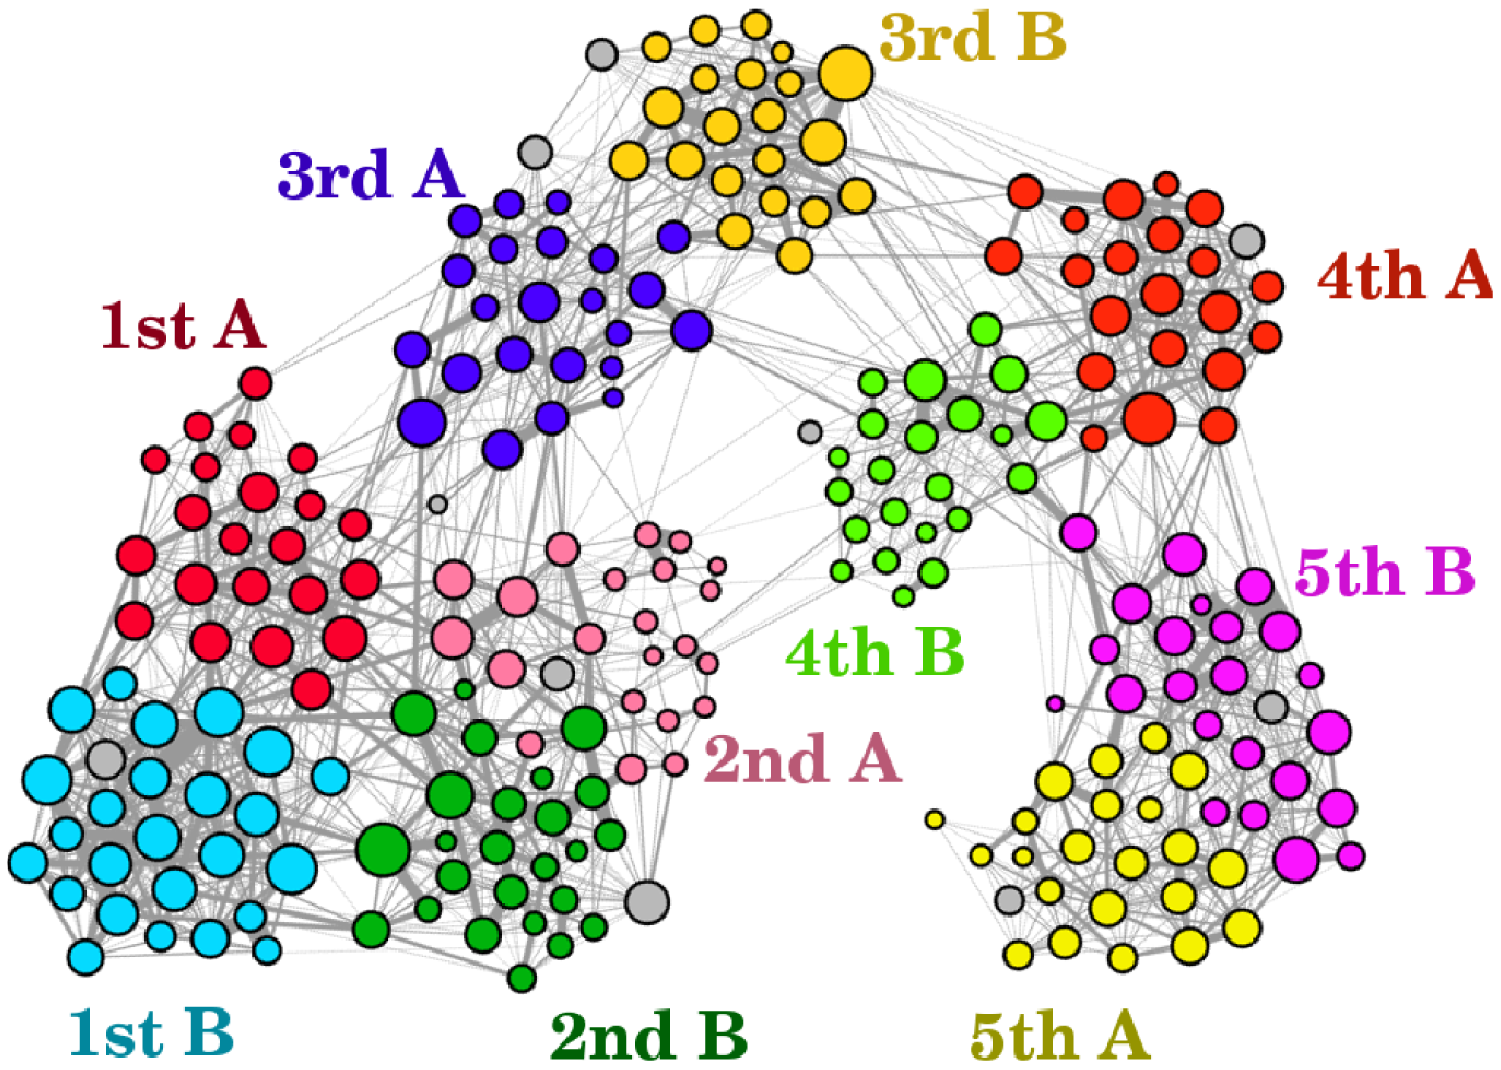
\includegraphics[width=0.7\linewidth]{img/Intro/ecole_primaire}
\caption{Graphe de contact des enfant d'une école primaire. L'épaisseur du lien représente la durée de communication entre deux élèves. La couleur représente la classe de chaque élèves. Les professeurs sont en gris.\protect\footnotemark}
\label{fig:ecole_primaire}
\end{figure}
\footnotetext{Image provenant de \url{http://journals.plos.org/plosone/article?id=10.1371/journal.pone.0023176}.}

Afin de capturer des partitions de n\oe uds, beaucoup de méthodes existent.
Il y a d'ailleurs régulièrement des état de l'art qui sont publiés~\cite{Fortunato2010,Plantie2013a, Malliaros2013a, Harenberg2014a}.
Afin d'aider le lecteur, nous détaillons ici quelques unes des méthodes les plus utilisées.

\subsubsection{Méthodes utilisant un modèle pour la comparaison}
\label{def:Modularite}
Comme une communauté est souvent définie comme devant être très connectée, le problème est de trouver une fonction capable d'évaluer la connexité d'une communauté.
Pour ce faire, deux \emph{ingrédients} sont nécessaires.
Tout d'abord, il faut définir une métrique qui mesure la connexité, \emph{e.g.} le nombre de liens dans un groupe.
Puis, il est nécessaire de définir comment utiliser la métrique pour considérer qu'un groupe est très connecté.
Il est possible d'utiliser une métrique en la normalisant par ses bornes minimum et maximum.
Avec cette métrique normalisée entre $0$ et $1$, un groupe est considéré comme très connectés si son évaluation est supérieur à un certain seuil.
Cette approche n'est cependant pas adaptée pour la recherche de communauté car elle ne tiens pas compte de la structure du graphe\,\footnote{C'est plus approprié dans la recherche des groupes les plus denses~\cite{Balalau2015}.}.
Prenons l'exemple du graphe constitué d'une clique et du nombre de liens comme métrique.
Le nombre de lien d'un groupe est normalisé par le nombre minimum de liens, $0$, et par le nombre de maximum de liens qui est obtenu par une clique.
Dans ce graphe, tout groupe de n\oe uds est également une clique et par conséquent tout groupe de n\oe uds a un évaluation parfaite de $1$.
Chaque groupe serait donc une très bonne communauté selon cette évaluation.
Or, le graphe constitué d'une unique clique ne possède pas de structure communautaire contrairement au graphe dans la figure~\ref{fig:ecole_primaire}.
Il est donc nécessaire de trouver une autre approche.

Plutôt que de normaliser une métrique par ces valeurs minimum et maximum, il est intéressant de considérer l 'écart à une valeur moyenne.
L'idée est la suivante: quelle serait la valeur attendue de la métrique considérée si le graphe n'avait pas de structure communautaire.
Le problème est alors de définir des graphes qui n'ont pas de structures communautaires.
L'ensemble des graphes similaires définit alors un \emph{modèle nul}.
Détecter des communautés se traduit alors en trouver des groupes qui s'éloignent du modèle nul considéré où il n'existe pas de communauté.
Ce changement est astucieux car il est relativement aisé de définir des graphes n'ayant pas de structure.
Il suffit de créer des graphes complètement aléatoires~\cite{Erdos1959} où les liens du graphes sont tirés de manière uniforme.
Afin que les graphes aléatoires puissent être comparable au graphe initiale, des contraintes sont généralement ajoutées et donnent lieu à différent modèle nul.
Le premier modèle nul de graphe est celui de Erdös-Rényi~\cite{Erdos1959} où le nombre de liens et le nombre de n\oe uds des graphes aléatoires doivent être les mêmes que dans le graphe initial.
Un autre modèle très couramment utilisé est le modèle de configuration~\cite{Bender1978a}.
Dans ce modèle, la distribution des degrés est également fixe.
Le modèle de configuration est souvent utilisé car il a été observé que les graphes provenant de données réelles ont une distribution des degrés très éloignés d'une distribution uniforme.
C'est pourquoi l'ajout de la contrainte dans le modèle nul sur les degrés permet de considérer des graphes plus similaire au graphe initiale. 
Ils existent bien évidement d'autres modèles possibles considérant d'autres contraintes~\cite{Newman2009}.

\paragraph{Modularité}
La modularité~\cite{Newman2004} est une fonction qui associe a chaque partition de n\oe uds une valeur de qualité entre $-1$ et $1$.
Plus la valeur de modularité d'une partition est élevée, plus la partition est censée capturer une structure communautaire.
La modularité est définie de la manière suivante pour une partition $\mathcal{C}$:

\begin{equation}
Q(\mathcal{C}) = \dfrac{1}{2M}\sum_{i,j \in V} \left(A_{ij} - \dfrac{d_id_j}{2M}\right)\ \delta_{C(i)=C(j)} \ .
\end{equation}
Il s'agit pour deux n\oe uds d'une même communauté de comparer la présence ou absence d'un lien,$A_{ij}$, à la probabilité que ces des n\oe uds soient reliés dans le modèle de configuration, $\dfrac{d_id_j}{2M}$.
L'idée sous-jacente est que les n\oe uds d'une communauté devraient partager plus de liens qu'espéré dans le modèle de configuration.
De très nombreux travaux ont par la suite étudié les caractéristiques de la modularité et son optimisation.
Tout d'abords, il a été montré que l'optimisation de la modularité est un problème NB-Complet~\cite{Brandes2007}.
Il est donc nécessaire de recourir à des heuristiques afin de trouver rapidement une partition proche de l'optimum
Parmi l'ensemble des algorithmes existant, l'algorithme de Louvain~\cite{Blondel2008a} est un des plus rapide.
Il existe également des variantes de cet algorithme~\cite{Huang2015,Traag2015a}.
D'autres travaux se sont attachés à l'étude de la modularité.
Il a été montré que la modularité souffre du problème de \emph{résolution limite}~\cite{Fortunato2007,Lancichinetti2011} car le modèle de configuration présuppose une répartition uniforme des tailles des communautés.
Il a par ailleurs été montré que la modularité n'offre pas de maximum clair et que beaucoup de partitions différentes ont des évaluations proches~\cite{Good2010}.
Pour répondre à ces problèmes, il existe des variantes~\cite{Reichardt2006,Delvenne2010}.

\paragraph{Surprise}
La fonction Surprise~\cite{Aldecoa2011,Traag2015b} est une autre fonction de qualité qui se base quant a elle sur le modèle de Erdös-Rényi pour évaluer la surprise d'observer un groupe de n\oe uds relié par $l$ liens.

\paragraph{Stochastic Block Model}
Nous avons définis précédemment la notion de modèle nul permettant de se comparer à l'absence de communautés.
Il est également possible de modéliser une structure communautaire puis de vérifier \emph{a posteriori} si ce modèle pourrait être à l'origine du graphe observé.
Le problème de détection de communauté est alors un problème d'inférence qui est traité avec des outils statistiques tel que le \emph{stochastic block model} (SBM)~\cite{Holland1983a,Nowicki2001}.
L'idée derrière le SBM est la suivante: la probabilité que deux n\oe uds soient reliés dépend uniquement de leur groupe respectif.
Si le graphe a une structure communautaire, alors deux n\oe uds d'une même communauté devraient avoir une forte chance d'être connecté.
\`A l'inverse, deux n\oe uds de deux communauté différentes devraient avoir une probabilité assez faible d'être connecté.
Le SBM est défini par de nombreux paramètres: le nombre de groupe, l'assignation d'un groupe à chaque n\oe ud et les probabilités d'interactions entre les groupes.
Avec un jeu de paramètres donné, il est alors possible de calculer la vraisemblance que ce jeu de paramètre soit à l'origine du graphe.
Trouver une partition de n\oe uds dans ce contexte est alors équivalent à trouver le jeu de paramètre qui est le plus vraisemblablement à l'origine du graphe.

Dans le SBM, tout les n\oe uds sont considérés comme équivalents en particulier vis-a-vis du degré ce qui n'est pas le cas dans beaucoup de graphes provenant de données réelles.
C'est pourquoi une version tenant compte du degré des n\oe uds a été proposée: le Degree-correcte Stochastic Block Model (DBSM)~\cite{Karrer2011}.
Enfin d'après de récents travaux\cite{Newman2016}, il semblerait que le DSBM et l'optimisation de la modularité soient liés.

\subsubsection{Méthodes utilisant des marches aléatoires}
Il existe de nombreuses autres approches que celles utilisant un modèle nul ou un modèle générateur.
Notamment, il y a des méthodes utilisant les marches aléatoires \cite{Pons2005,Rosvall2008}.
Ces méthodes tirent partis du fait que si une communauté est densément connectée alors un marcheur aléatoire devrait y rester assez longtemps.
En particulier, la méthode Infomap~\cite{Rosvall2008} repose sur une idée très élégante; une partition de n\oe uds est une carte du graphe et, en ce sens, elle doit aider sa lecture.
Une carte est efficace si elle permet de mieux comprendre l'objet d'étude en réduisant sa complexité.
Dans une carte d'un pays, les départements découpent l'espace en zones compactes et la plupart du temps la majorité des routes se retrouvent à l'intérieur des départements.
Ainsi un voyageur se déplaçant aléatoirement sur les routes a peu de chance de sortir d'un département.
Pour décrire, \emph{a posteriori}, l'ensemble des routes prises par ce voyageur, il suffit alors de donner le département initiale puis la liste des routes empruntées.
Il n'est pas nécessaire de répéter le département à chaque fois si le voyageur n'en est pas sortit.
En ce sens, la découpe d'un pays en département permet de réduire la complexité du voyage.
Il s'agit donc d'un problème lié à la théorie de l'information et de sa compression.
De manière similaire, Rosval~\emph{et al.} utilise des marcheurs aléatoires se déplaçant sur les n\oe uds du graphe et les communautés forment des zones du graphe.
Si les communautés sont bien formées et que les marcheurs aléatoires restent bloqués à l'intérieur, alors la description de leur marche aléatoire sera courte.
La longueur de cette description devient alors la signature de la partition et plus la signature est courte, meilleur la partition est.

La méthode a également été étudiée pour voir si elle souffre de \emph{résolution limite} comme la modularité~\cite{Kawamoto2015}.
Il semble que cet effet existe également dans Infomap mais qu'il soit beaucoup moins prononcé.

\paragraph{Autres méthodes}
Il existe bien d'autres méthodes pour détecter des communautés en tant que partition de n\oe uds.
Il y a les méthodes spectrales~\cite{Donetti2004,Mitrovic2009} qui se base sur les vecteurs propres de la représentation d'un graphe sous la forme d'une matrice.
De manière moins formelle, les méthodes sont des algorithme de propagations de labels (LPA)~\cite{Raghavan2007a,Li2014c}.
Dans ces méthodes, chaque n\oe uds a initialement un label puis à chaque itération chaque n\oe ud prend comme label un des label de ses voisins.
En général, un n\oe ud prend comme label celui qui est le plus présent parmi ses voisins.
Au bout d'un certain nombre d'itération ou l'équilibre, il ne reste que beaucoup moins de labels qui représentent les communautés.


\resume{Il existe de très nombreuses méthodes pour la détection de communautés en tant que partition de n\oe uds. Ils semblent que les méthodes d'optimisation de \textbf{modularité}, la méthode \textbf{infomap} et  les \textbf{Stochastic Block Model} soient les plus utilisées dans la littérature.}

\subsection{Couverture de n\oe uds}
\label{subsec:cover}
Jusqu'à maintenant nous avons considérons les communautés comme des partition de n\oe uds.
Or, les partitions sont très restrictives et ne peuvent pas capturer toutes les situations possibles.
Reprenons l'exemple d'un graphe reflétant des interactions de personnes comme dans la section~\ref{sec:intro_communaute}.
Ils existent des communautés qui sont disjointes comme le travail et la famille mais bien souvent des personnes appartenant à plusieurs groupes, voir l'exemple dans la figure~\ref{fig:ex_overlap_communaute}.
Ainsi le groupe de personnes faisant du sport ensemble et le groupe des personnes travaillant ensemble peuvent ne pas être disjoint.
Si tel est le cas, alors il n'est plus possible de représenter des communautés avec une partition.
Il est nécessaire de manipuler une couverture de n\oe uds.
Ainsi dans l'exemple dans la figure~\ref{fig:ex_overlap_communaute}, les n\oe uds rouges devraient appartenir deux groupes au lieu d'un seul.

\begin{figure}
	\centering
	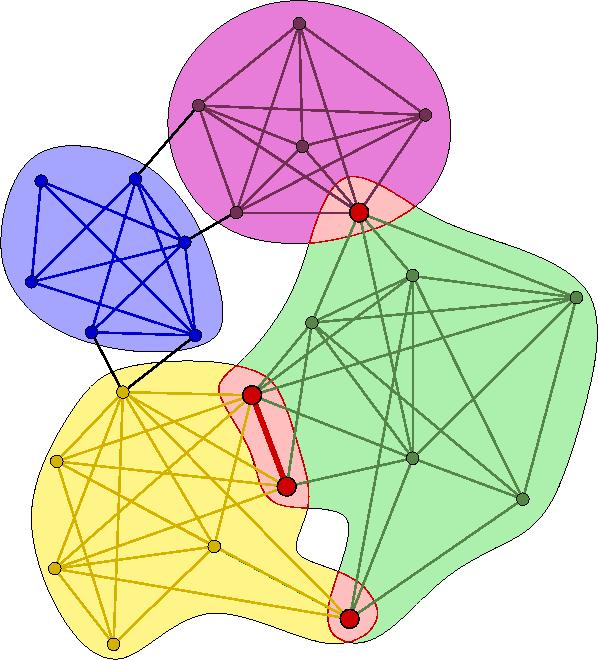
\includegraphics[width=0.31\linewidth]{img/Intro/Illustration_of_overlapping_communities.jpg}
	\caption{Exemple graphe avec une structure communautaire chevauchante représenté par les couleurs\,\protect\footnotemark.}
	\label{fig:ex_overlap_communaute}
\end{figure}
\footnotetext{Image provenant de \url{https://en.wikipedia.org/wiki/Clique_percolation_method}.}

Une fois encore, la littérature est très vaste dans ce domaine et nous ne ferons pas une liste exhaustive des méthodes existantes.
Pour une liste plus exhaustive, il existe de nombreux état-de-l'art dans le domaine~\cite{Danisch2012, Kanawati2014, Xie2013,Bandyopadhyay2015, Hric2014a}.

Une des premières méthodes de détection de couverture de n\oe uds est la \emph{Clique Percolation Method} (CPM)~\cite{Palla2005}.
L'algorithme CPM repose sur le principe de transitivité qui serait à l'origine des communautés: si $i$ et $j$ sont reliés par un lien alors le n\oe ud $k$ qui est déjà relié à $i$ a une forte chance d'être également connecté à $k$.
Il s'agit de la formalisation du proverbe "Les amis de mes amis sont mes amis".
Si ce principe est réellement à l'origine des communautés, alors elles doivent être composées de plusieurs cliques.
C'est pourquoi CPM cherche l'ensemble des cliques d'une taille $k$ donnée, en générale $k<10$ pour des raisons de coût de calcul, puis fusionne toutes les cliques qui partagent suffisamment de n\oe uds, en générale $k-1$. 
Comme cette méthode est relativement couteuse, Kumpula \emph{et al.}~\cite{Kumpula2008} ont repris le même mécanisme en optimisant le mode de calcul.

\subsubsection{Extension de méthodes existantes}

La majorité des méthodes existantes pour les partitions ont été adaptées pour manipuler les couvertures de n\oe uds.
Il existe plusieurs extensions de la modularité~\cite{Shen2009,Nicosia2009}.
Cependant ces extensions ne reposent plus sur un modèle nul car elles introduisent des termes de normalisations.
Par conséquent, ces extensions sont beaucoup moins utilisées que la modularité initiale.

\paragraph{Stochastic Block Model}
En revanche, le SBM s'adapte très bien aux couvertures de n\oe uds.
Une extension du SBM est le Mix-Membership Stochastic Block Model (MMSBM)\cite{Airoldi2008} qui permet à un n\oe uds d'avoir plusieurs groupes.
Dans~\cite{Gopalan2013a}, les auteurs utilisent la même méthodes mais en échantillonnant le graphe initiale afin de réduire le cout de calcul.
Il existe d'autres méthodes à base de modèle génératif~\cite{Ball2011,Yang2013}.
Ces méthodes se basent sur des graphe d'affiliation\cite{BreigerRonald1974}.
Un graphe d'affiliation est un graphe biparti entre les n\oe uds d'une part et les communautés de l'autre part.
Dans la méthode de Ball\emph{et al.}, ce graphe d'affiliation est pondéré et la pondération représente la propension d'un n\oe uds à créer des liens dans un groupe donné tant dis que dans Yang\emph{et al.} il s'agit du facteur d'appartenance du n\oe uds au groupe.
Une fois le graphe d'affiliation définit, il est nécessaire de savoir recréer la matrice d'adjacence et, en ce sens, ces méthodes se rapprochent des méthodes de factorisation non négative de matrices~\cite{Lee1999}.
Le but de la factorisation non-négative d'une matrice donnée est d'être capable de trouver deux matrices dont les entrées sont non-négatives tel que leur combinaison permettre de retrouver la matrice initiale.

Jusque récemment ce genre de technique généralisant le SBM ne pouvaient s'appliquer qu'à des graphes relativement petit.
il semble cependant que les méthodes récentes~\cite{Gopalan2013a, Yang2013} arrivent à traiter des graphes ayant énormément de liens, de l'ordre $10^{12}$ liens.



\paragraph{Propagation de label}
Des méthodes ont étendus la propagation de label aux couvertures de n\oe uds~\cite{Gregory2010,Xie2011}.
Le principal changement est qu'un n\oe ud ne stocke plus un unique label mais soit plusieurs labels soit des fréquences d'apparition de label.
Ainsi à la fin de l'algorithme, il suffit de choisir les labels les plus fréquents.
Cependant ce mécanisme de propagation change radicalement de l'idée initiale.
En effet, la diffusion d'un label n'est plus directement contrainte par la diffusion des autres labels.
Dans cette nouvelle configuration, il est possible qu'un label soit présent dans tout les n\oe uds.
De plus selon les auteurs de ces méthodes, des communautés non connexes peuvent apparaître ce qui nécessite l’ajout d’un mécanisme de post-processing.


\paragraph{Infomap}
Il s'agit surement de la méthode étant le moins "déformé" avec le SBM par l'adaptation aux partitions chevauchantes.
En effet, il suffit de relâcher la contrainte sur le fait qu'un n\oe ud n'appartienne qu'à un seul groupe.
Il est toujours possible de décrire un trajet par un nom de groupe puis une liste de n\oe uds visités dans le même groupe.
Ainsi, la notion de longueur de description est toujours valide même dans contexte.
Ce travail d'extension a été fait par Esquivel\emph{et al.}~\cite{Esquivel2011}.

\subsubsection{Méthodes utilisant des fonctions de qualité locales}
On a vu avec la modularité qu'il est assez difficile de définir une fonction de qualité évaluant une couverture de n\oe uds en fonctions des caractéristiques des groupes.
En revanche, les LPA tirent partis de l'information locale pour créer des groupes locales mais ne permettent pas leur évaluation.
L'idée est en quelque sorte mélanger ces deux aspects.
Il s'agit d'algorithmes qui initialement considèrent de très petites communautés puis essayent de les étendre itérativement en ajoutant des n\oe uds.
Afin de ne s'étendre un groupe indéfiniment comme cela peut être le cas avec les LPA, un ajout n'est fait que s'il améliore une fonction de qualité locale.
Ainsi dans ce type d'algorithme, il y a principalement deux critères important:
le choix des communautés initiales et le critère d'évaluation.
Dans la majorité des cas, chaque n\oe ud constitue une communauté. 
OSLOM\cite{Lancichinetti2011a} diffère de cette situation car OSLOM utilise comme point de départ une partition trouvée par l'algorithme de Louvain ou par infomap.

Les fonctions de qualité applicable sont très nombreuses et nous ne mentionneront que trois.
Tout d'abord, il est possible d'utiliser le degré relatif~\cite{Luo2008} d'un groupe comme critère.
Il s'agit du ratio entre le nombre de $l_{in}$ liens internes à un groupe de n\oe uds et du nombre de liens totale $l_{in}+l_{out}$:$ \dfrac{l_{in}}{l_{in}+l_{out}}$.
En effet, plus le degré relatif est élevé, plus le groupe est dense comparé à son voisinage et plus il a de forte chance d'être une bonne communauté. 
Cette formulation est assez proche de la conductance ou coupe normalisée\cite{Shi2000}:
\begin{equation}
\phi =\dfrac{l_{out}}{\min \left( 2(l_{in}+l_{out}),m-2(l_{in}-l_{out}) \right) }
\end{equation}

Ces deux notions se rapportent à la notion de densité vis-à-vis de leur voisinage.
Il également possible d'évaluer une communauté locale par rapport aux nombre de triangles présents de la communauté.
C'est ce que mesure la cohesion~\cite{Friggeri2011} pour un groupe de taille $k$: 
\begin{equation}
cohesion=\dfrac{\Delta_3}{ {k \choose 3} } \times \frac{\Delta_3}{\Delta_3+\Delta_2},
\end{equation}
où $\Delta_3$ est le nombre de triangle dont les 3 n\oe uds sont à l'intérieur du groupe et $\Delta_2$ est le nombre de triangle dont unqiement 2 n\oe uds sont à l'intérieur du groupe.

Différentes méthodes d'initialisation ainsi que fonctions de qualité sont déaillées dans l'article de Kanawati~\cite{Kanawati2014}.
Ces méthodes semblent très prometteuses car elles permettent de traiter efficacement de très grand graphe tout comme les LPA mais elles profitent des fonctions de qualité locales qui permettent d'une certaines manières d'évaluer le résultat obtenus.


\resume{
La littérature sur la détection de couverture de n\oe ud est encore très récente.
Il est donc délicat de commencer à tirer des conclusions.
Cependant, il semble que les extensions de la modularité ne soient pas réellement capable de trouver des couvertures de n\oe uds.
En plus d'infomap, c'est surtout les méthodes utilisant des modèles génératifs et celles utilisant des fonctions de qualité locales qui semblent les plus à même de capturer des couvertures de n\oe uds pertinentes.
Bien que souvent limité à de petit exemple, les modèles génératifs semblent maintenant capable de traiter des graphes de tailles importantes.
Les méthodes utilisant des fonctions de qualité locales sont quant à elle très rapide mais le choix de la fonction de qualité semble encore délicat.
}


\section{Extension temporelle des graphes}
\label{sec:intro_extension_temporelle}

Les graphes sont utilisés pour représenter une situation ou résoudre un problème réel.
Dans le chapitre précédent, nous nous sommes attachés à présenter une partie des méthodes considérant le problème de la détection de communautés recouvrantes ou non.
Cependant toutes ces méthodes reposent sur la validité de la représentation du problème par un graphe.
Cette hypothèse est justifiée dans énormément de cas.
Ce n'est par contre pas le cas lorsque l'objet d'étude évolue durant la capture.

Afin d'illustrer ce propos, nous appuyons sur le même exemple de réseau de personnes que nous avons présenté dans la sous-section~\ref{subsec:Part_noeuds} et qui est illustré dans la figure~\ref{fig:ecole_primaire}.
Dans cet exemple, deux élèves sont reliés dans le graphe si ils ont interagis au moins une fois au cours de la capture.
Dans ce cas, on parle de graphe agrégé car la dimension temporelle est complètement oubliée.
Comme la capture n'a duré que deux jours, il est fort probable que les élèves n'aient pas changé d'habitude durant la capture.
En étudiant le graphe agrégé, il est possible de mettre en avant l'organisation générale des élèves mais déjà de l'information a été perdue.
En effet, il n'est pas possible de différencier le comportement observé le matin de celui observé le soir car l'ensemble des interactions sont agrégées dans le graphe.
Ce n'est pas tout, imaginons que la capture ait duré plusieurs mois voir plusieurs années.
Dans ce cas de figure, il ne sera plus possible de dégager un comportement général des élèves car ils auront changé durant ce laps de temps.
En particulier, de nouveaux groupes d'amis se seront formés et d'autres auront disparu.
Tout ces changements impactent le graphe agrégé et tendent au fur et à mesure à le rapprocher à une grande clique ce qui le rend complètement inexploitable.
Le temps est donc une dimension qu'il est nécessaire de prendre en compte.

Le domaine de l'épidémiologie sont de très bon exemples de l'importance du temps.
Un modèle épidémique modélise la propagation d'une maladie dans une population en fonction des contacts qui existent.
Il est donc tout naturel de s'appuyer initialement sur un graphe où les n\oe uds représentent des personnes et les liens représentent les interaction entre personnes.
En plus du graphe, il est nécessaire d'ajouter l'états de chaque n\oe uds, \emph{e.g.} n\oe ud sain ou n\oe ud infecté.
Ainsi, un n\oe ud sain ne peut devenir infecté que s'il est relié à un n\oe ud infecté dans le graphe.
Ce genre de modèle mettent donc en avant un chemin de diffusions, \emph{e.g.} une suite de personnes transmettant sa maladie à l'autre.

Afin d'illustrer ce phénomène, les premiers travaux~\cite{Vespignani2008}
s'appuient sur un graphe d'interaction de personnes agrégeant toute l'information temporelle.
Or, la prise en compte du temps dans ce contexte est primordiale car il est possible que le chemin d'infections simulé dans le graphe agrégé ne soit pas réalisable si l'on prend en compte le temps.
Imaginons 3 personnes $A$, $B$, $C$ tel que $A$ et $B$ interagisse à l'instant $1$, $B$ et $C$ interagisse à l'instant $2$.
Dans le graphe agrégé, il est possible pour $C$ d'infecter $A$ via $B$ alors que dans la réalité cela n'est possible.
L'ajout du temps impacte donc fortement les résultats obtenus dans le contexte épidémiologique et ce phénomène est d'ailleurs très étudié~\cite{Gauvin2015,Karsai2011,Jo2014,Horvath2014,Holme2014a,Scholtes2014,Perotti2014}.

Une fois reconnue l'importance du temps, il est nécessaire de trouver un nouveau formalisme étendant la théorie des graphes pour tenir compte du temps.
Nous présentons maintenant différentes extensions possibles de la théorie des graphes, dans les sous-sections~\ref{subsec:perte_info} et \ref{subsec:pasperte_info}.
Nous détaillons également comment la recherche de communautés se transpose dans ces nouveaux formalismes et plus généralement quelles sont les problèmes qu'ils permettent de résoudre.
Des états de l'art dans ce domaine ont d'ailleurs déjà été esquissés~\cite{Boccaletti2014,Cazabet2014,hartmann2014clustering}.

\subsection{Extensions avec pertes d'informations temporelles}
\label{subsec:perte_info}
\subsubsection{Séries de graphes}
\begin{figure}[h]
\centering
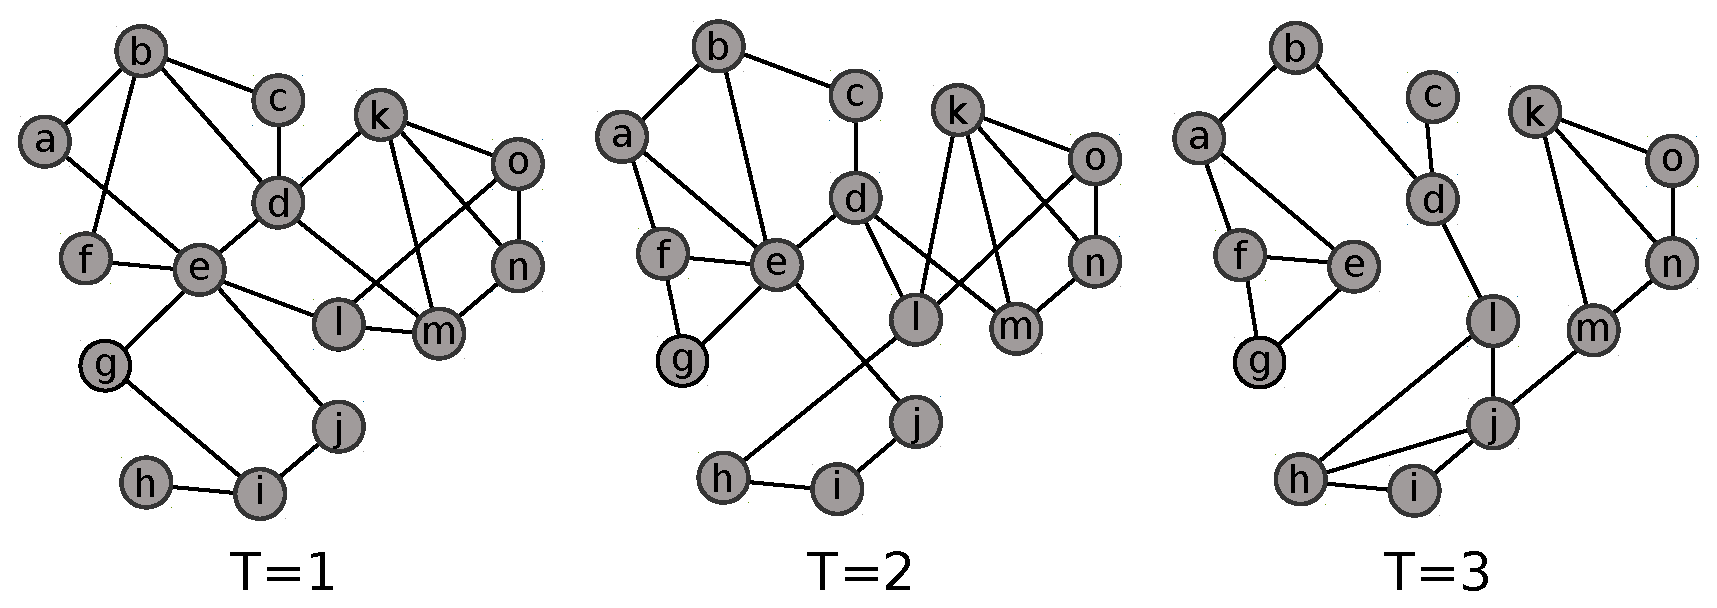
\includegraphics[width=0.8\linewidth]{img/Intro/TVG.eps}
\caption{Exemple de série de graphes sur trois intervalles de temps.}
\label{fig:exemple_TVG}
\end{figure}
La première solution qui a été apportée ne prends le temps en compte que partiellement.
Il s'agit de manipuler une série de graphe où chaque graphe représente le système durant un intervalle de temps donné.
Ainsi, il est possible d'appliquer les outils de la théorie des graphes sur chaque intervalle de temps.
Cependant chaque intervalle de temps est représenté par un graphe agrégé.
Il y a donc une perte d'information.
Plus formellement, une série de graphe est défini par $\mathcal{G}=\{G_i\}_{i < T}$ où $T$ est un entier, voir l'illustration~\ref{fig:exemple_TVG}.

Cette définition initiale laisse le choix sur la découpe du temps en intervalle.
Il est possible de choisir des intervalles de tailler égale ou non et disjoints ou chevauchant\cite{Wang2012}.
Utiliser des intervalles à durée variable permet de mieux tenir compte de la dynamique.
Par exemple lors de l'étude d'interactions de personnes, il est très courant d'observer une très faible activité la nuit et une plus forte le soir.
Un graphe agrégeant ce qui se passe sur un intervalle de 5h sera vide dans le premier cas et peut être trop dense dans le second.
La détection d'intervalle pertinent est donc un vaste sujet de recherche~\cite{Rosvall2010,Krings2012,Ribeiro2013,Caceres2013,Peel2015,de2016detection}.

La notion même de temps est importante.
Albano \emph{et al.}~\cite{Albano2014} propose même d'utiliser une autre mesure que la seconde ou la journée mais plutôt le nombre de changement comme mesure du temps.
Ainsi, le temps n'avance pas si aucun changement n'a lieu et au contraire il avance beaucoup si énormément de changement apparaissent.
Cette manière de procéder se rapproche des travaux de Lamport~\cite{Lamport1978} dans les système distribués.

\paragraph{Détection de communautés}
Dans ce contexte de série de graphe, il y a eu assez tôt des méthodes de détection de communautés~\cite{Hopcroft2004,Sun2007,Lin2008,Asur2009}.
Il est, en effet, assez naturel d'appliquer une méthode de détection statique sur chaque graphe puis d'essayer de faire du suivie de communautés.
Le suivi de communauté consiste en étant une série de graphe et une série de partition comprendre comme un communauté donnée à évoluer.
Palla \emph{et al.}~\cite{Palla2007} ont été parmi les premier à décrire les évolution possible d'une communauté.
Muni d'indicateur de similarité tel que l'indice de Jaccard, voir~\ref{def:graphe_comparaison}, il est possible de trouver les communautés les plus proches aux instant précédant et suivant.
\`A partir de ces informations, il est défini 5 type d'évolutions d'une communauté:
\begin{description}
\item[Naissance] il n'existait pas de communauté proche précédemment.
\item[Agrandissement] La communauté continue d'exister et s'agrandit.
\item[Fusion] Deux communautés fusionnent pour donner lieu à une nouvelle communauté.
\item[Division] Une communauté se sépare en deux nouvelles communautés à l'étape suivante.
\item[Mort] Une communauté cesse d'exister dans les graphes suivants.
\end{description}

Ce type de méthode souffre souvent de l'instabilité des méthodes de détections~\cite{Aynaud2010,Harenberg2014a}.
Si les partitions changent complètement entre deux graphes consécutif, alors il est difficile de faire un réel suivi de communautés.
C'est pourquoi des méthodes essayent de forcer une certaine stabilité de la partition en ajoutant un coût de transition~\cite{Chakrabarti2006,Chen2013,Kalavathi2015}.
Une approche détournée pour garder une certaine stabilité est d'utiliser la partition trouvé précédemment comme base de recherche pour l'intervalle suivant~\cite{Lancichinetti2011a}.

Des extensions du Stochastic Block Models ont également étaient proposés par différents auteurs dans le cadre des séries de graphes.
Yang~\emph{et al.}~\cite{Yang2011} est parmi les premier à considérer ce cas de figure.
Ils considèrent que le nombre de liens partagé par une pair de communauté est fixe et que ce qui change est l'affiliation d'un n\oe uds à une communauté.
Ce processus de changement de communauté suit une chaine de markov cachée.
\`A l'inverce, Corneli~\emph{et al.}~\cite{Corneli2016} considèrent le cas opposé.
La partition de n\oe uds est fixe tout au long du temps et c'est l'activité entre deux communauté qui change selon l'intervalle de temps.
Xu~\emph{et al.}~\cite{Xu2014} permettent à l'affiliation et à l'activité entre deux communautés de changer selon l'intervalle de temps.
Cependant, il semblerait que cette relaxation se fasse au dépens de l'identifiabilité des paramètres d'après Matias~\emph{et al.}~\cite{Matias2015}.
Ils ont donc proposé une nouvelle méthode afin résoudre ce problème.
De plus, leur méthode permet de traiter des séries de graphes pondérés.

\subsubsection{Tenseur 3D}
Les tenseurs 3D ne sont pas en soi différent des séries de graphes.
Il est possible de voir un graphe comme une matrice carré d'adjacence.
Il est donc normal de concevoir une série de graphe comme un tenseur appartenant à $\mathcal{R}_{nnT}$.
Ce changement de point de vue permet ainsi d'appliquer les méthodes d'algèbre linéaire, notamment la décomposition de tenseur.
C'est la méthode proposée par Gauvin~\emph{et al.}~\cite{Gauvin2014} pour étudier la structure communautaire des interactions d'élèves.



\subsubsection{Graphes multicouche}
\begin{figure}[h]
\centering
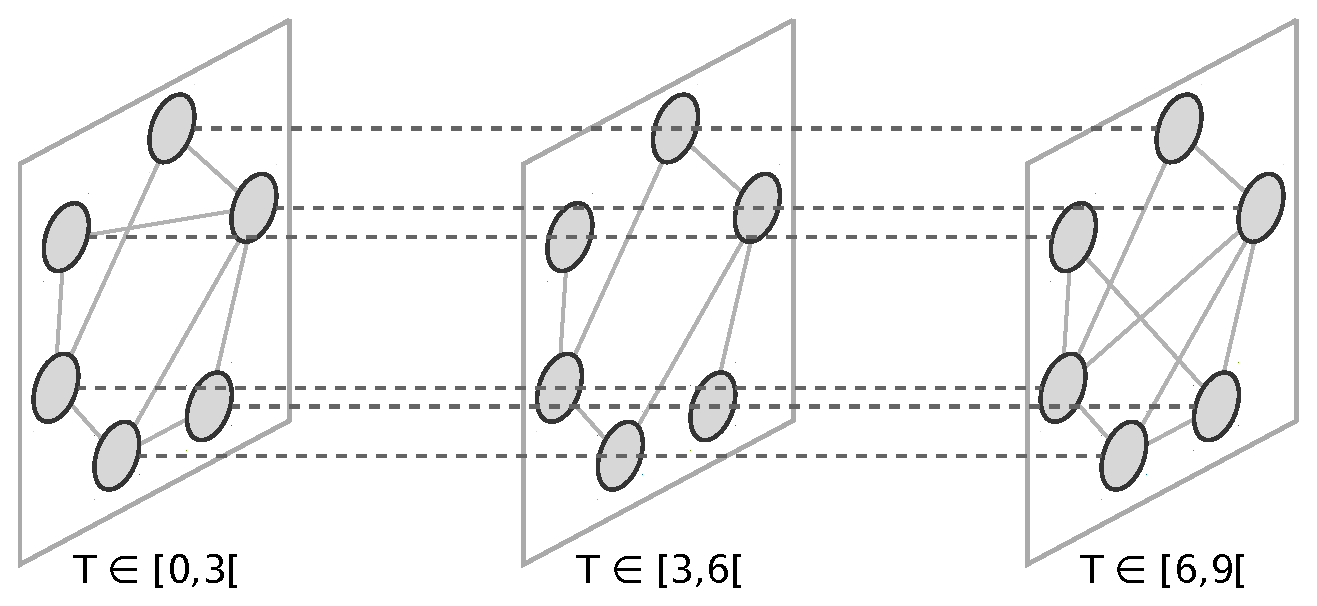
\includegraphics[width=0.7\linewidth]{img/Intro/multiplex.eps}
\caption{Graphe multicouche avec trois couches représentant le temps.
Les liens pleins (resp. pointillés) sont les liens intra-couches (resp. inter-couches).}
\label{fig:exemple_multiplex}
\end{figure}
La construction de graphes multicouche (\emph{multilayer} ou \emph{multiplex}) est proche de l'idée des séries de graphes.
Tout comme les séries de graphes, des n\oe uds et des liens sont créés à chaque intervalle pour représenter ce qui s'est déroulé l'intervalle de temps.
Cependant, le graphe multicouche ajoute des liens entre les n\oe uds de deux intervalles si'ls sont identiques, voir l'illustration~\ref{fig:exemple_multiplex}.
Par conséquent, un graphe multicouche est un graphe où il existe deux type de liens dans un graphe multicouche: les liens intra-couches et les liens inter-couches.
Les liens intra-couches représentent un connexion entre entre deux n\oe uds durant un intervalle de temps.
Les liens inter-couches représentent un lien entre deux n\oe uds sur deux intervalles différents.
Ces derniers sont utilisés pour identifier un même n\oe ud sur plusieurs intervalles et sont en générales limités à relier deux couches consécutives.

Les graphes multicouches représentent très bien les donnée évoluant dans le temps mais ils modélisent aussi très bien d'autres situations.
Par exemple, ils permettent de représenter facilement les différent moyens de transport dans une ville où chaque moyen de transport (bus, voiture, métro ...) est représenté par une couche.
Plusieurs travaux~\cite{DeDomenico2013,Kivela2014,Boccaletti2014} décrivent les graphes multicouches et leurs applications.



\paragraph{Détection de communautés}
Grâce au formalisme de graphe multicouche, il est possible de traiter le temps de manière un peu plus fine que dans les séries de graphes car il permet de mieux suivre l'évolution des n\oe uds.
Comme un graphe multicouche est un graphe, il est possible d'adapter les méthodes existantes pour tenir compte des différents type de liens.
C'est le cas d'infomap~\cite{DeDomenico2014}, de la modularité~\cite{Mucha2010,Bassett2013,Bazzi2016} et du SBM~\cite{Stanley2015,Peixoto2015c}.


\resume{
Les séries de graphes, les tenseurs et les graphes multicouches permettent de prendre en compte le temps tout en autorisant l'utilisation de méthode conçu sur un graphe statique.
Cette liberté d'utilisation a un coût.
Ces approches reposent sur une découpe du temps en sous-intervalles durant lesquelles le temps n'est plus pris en compte afin d'obtenir un graphe statique.
Il peut être délicat de définir un intervalle de temps qui permet de construire des graphes qui aient du sens.
La construction des graphes agrégés entraine une perte d'information temporelle et cela impacte la précision temporelle des structures communautaires qui sont manipulables.
Il n'est pas envisageable d'augmenter le nombre d'intervalle de temps car cela induirait d'une part des graphes agrégés avec très peu de liens et d'autre part le temps de calcul serait très fortement impacté.
}

\subsection{Extension sans perte d'information temporelle}
\label{subsec:pasperte_info}
\subsubsection{Graphe temporel}
\begin{figure}[h]
\centering
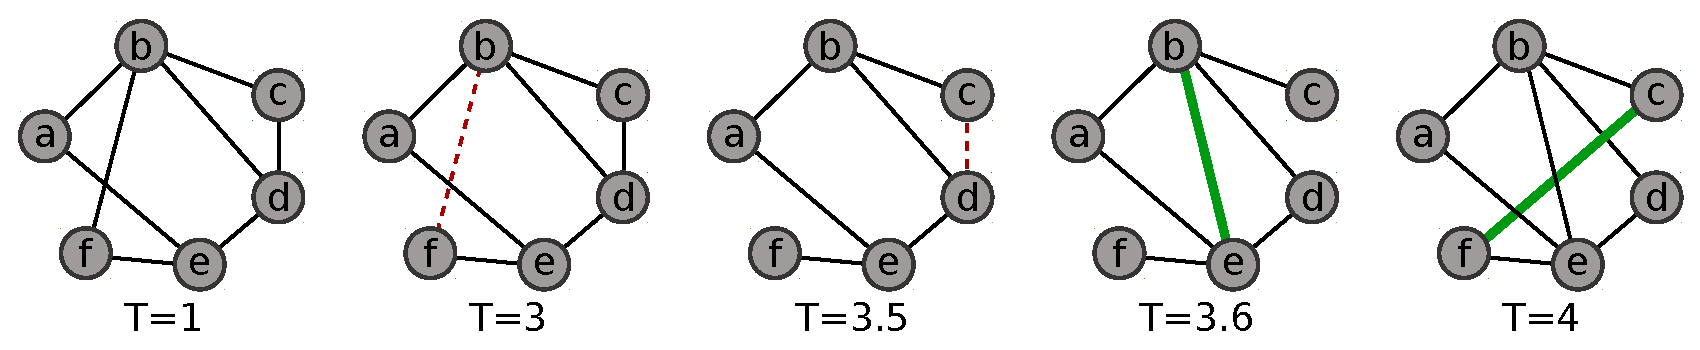
\includegraphics[width=0.9\linewidth]{img/Intro/evolvingGraph.eps}
\caption{Graphe temporel avec des ajouts de lien représentés en trait épais vert et des retraits de lien représentés par des liens pointillés rouge.
}
\label{fig:exemple_evolving}
\end{figure}
Les graphes temporels (\emph{Time Varying Graph} ou \emph{Evolving Graph})
permettent de tenir compte de l'ensemble de l'information temporelle.
Pour cela au lieu de considérer des intervalles de temps, ils considèrent l'ensemble des modifications qui affectent le graphe: les ajouts et retraits de liens.
En pratique, cela revient à considérer sur chaque lien une fonction de la présence en fonction de temps qui vaut $1$ à un instant $t$ si le lien existe à cet instant et $0$ sinon.
Ainsi, il est possible de connaitre la structure de graphe à chaque instant.
Ce formalisme est présenté dans différents travaux~\cite{Casteigts2011,Wehmuth2014} et illustré dans la figure~\ref{fig:exemple_evolving}.
Dans cette figure, on voit apparaitre l'ordre de modification du graphe.
Tout d'abord, les lien $(b,f)$ et $(c,d)$ disparaissent puis les liens $(b,e)$ et $(f,c)$ apparaissent chacun leur tour. 

\paragraph{Détection de communautés}
Dans un graphe temporel, une structure de graphe existe à chaque instant.
Il est donc possible de calculer après chaque modification l'évolution d'une métrique.
Par exemple, il est possible de calculer après l'ajout d'un lien le nouveau degré interne des n\oe uds impacté par ce changement..
En fonction de l'évolution de cette métrique, il est alors décidé d'ajouter ou retirer un n\oe ud voir même de fusionner deux communautés.
Li \emph{et al.}~\cite{Li2012a} se base sur le nombre de liens que partage un n\oe uds avec les communautés environnantes.
Ainsi, un n\oe ud est toujours dans la communauté avec laquelle il partage le plus de liens.
Shang\emph{et al.}~\cite{Shang2014a}, Cordeiro~\emph{et al.}~\cite{Cordeiro2016} et Sun\emph{et al.}~\cite{Sun2014} se basent sur l'évolution de la modularité.
Cependant, ces approches ne permettent pas l'ensemble des évolutions possibles de communauté, en particulier l'apparition d'une nouvelle communauté.
C'est pourquoi l'évolution de la structure courante peut mener à une structure ayant une faible qualité.
Une autre approche a été proposée par Cazabet~\emph{et al.}~\cite{Cazabet2010} afin d'améliorer l'évolution de la partition.
ils utilisent sur une métrique locale basé sur le nombre de chemins de longueur $2$ existant entre un n\oe ud et une communauté.
Après chaque modification, ils considèrent également la possibilité de créer une nouvelle communauté sous la forme d'une petite clique.
Ainsi, ils assurent une meilleur qualité de la partition au cours de l'évolution.


\subsubsection{Flot de liens}
\begin{figure}[h]
\centering
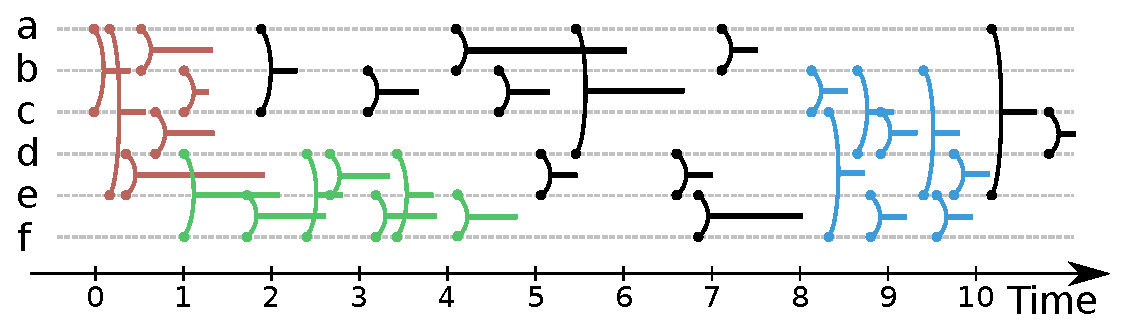
\includegraphics[width=0.9\linewidth]{img/Intro/Flot_de_liens.eps}
\caption{...}
\label{fig:exemple_Flot_de_liens}
\end{figure}
Dans les graphes temporels, toute l'information temporelle est gardée.
Cependant, l'idéologie derrière cette méthode est qu'il existe une structure de graphe à chaque instant.
Cette hypothèse n'est pas toujours vérifiée, en particulier lorsque les liens apparaissent et disparaissent très rapidement.
C'est le cas des appels téléphoniques qui durent rarement plus d'une heure ou bien de manière plus frappante les SMS et les courriels qui n'ont même pas de durées.
Dans ces contextes, il n'est pas possible d'assumer qu'à chaque instant une structure de graphe existe.
Il faut donc un formalisme et des mesures qui s'adaptent à ce contexte.
C'est pour répondre à ce besoin que le formalisme de flot de liens a été pensé.
Le but est de construire un objet ne présupposant aucune structure et qui stocke toute l'information disponible.


Prenons l'exemple des appels téléphoniques.
Les informations disponibles sont les appels, c'est-à-dire qui parle avec qui à quelle heure et pendant combien de temps.
Un appel peut donc être représenté par un quadruplet $(b,e,u,v)$ où $b$ (res. $e$) est le début (resp. la fin) de l'appel et $u$ et $v$ représentent des personnes.
Il est donc possible de modéliser des appels téléphoniques par un ensemble de quadruplet.
En faisant cela, aucune information n'est perdue et, en ce sens, flots de liens et graphes temporels sont équivalent. 
Cependant, ce changement de perspective induit une réflexion différente selon le formalisme considéré.

Les différences dans les méthodes de représentation des graphes temporels~\ref{fig:exemple_evolving} et celle des flots de liens~\ref{fig:exemple_Flot_de_liens} illustrent bien ce changement de perspective, bien que les deux figures ne représentent pas la même information.
Dans l'exemple de la figure~\ref{fig:exemple_Flot_de_liens}, les n\oe uds sont représentés sur l'axe des ordonnées et le temps sur l'axe des abscisses.
Un lien dans cette visualisation est représenté par un arc verticale reliant deux axes de n\oe uds et un trait horizontale représentant la durée.
Ainsi dans l'exemple, il existe un lien entre les n\oe uds $a$ et $b$ dans l'intervalle $[4,6]$.
Dans un graphe temporel, on abordera plus souvent les questions d'évolution de communautés de n\oe uds ou de l'importance d'un n\oe ud.
Dans un flot de liens, on s'intéressera plus souvent au temps nécessaire pour que deux n\oe uds soient de nouveau en contact ou à l'importance d'un lien.
De manière très manichéenne et inexacte, le formalisme de graphe temporel pousse à étudier les n\oe uds et leur évolution alors que celui de flot de liens mets plus l'accent sur les liens.


Plusieurs travaux~\cite{Holme2013a,Holme2015b,Holme2015} font un tour d'horizon des méthodes existantes pour étudier des flots de liens qui sont souvent appelés \emph{temporal networks}.
Il existe, à notre connaissance, qu'un seul travail donnant un fondement théorique solide.
Il s'agit de Batagel~\emph{et al.}~\cite{Batagelj2015} qui se basent sur l'algèbre et donc les notions de chemins semblent difficile à représenter dans ce contexte pour l'instant.\bigskip


Avec ce formalisme, la majorité des travaux sont encore descriptifs car ce type d'objet n'a jamais été étudié sous cet angle.
Il existe de nombreux travaux étudiant le temps séparant l'apparition de deux liens pour un n\oe uds~\cite{Malmgren2008,Malmgren2009}.
Il semblerait que ces temps inter-contacts soient très hétérogène avec de nombreuses connexions dans un faible intervalle de temps suivie de longue durée sans activité.
On parle alors de temps inter-contact \emph{bursty}.
Les effets des temps inter-contacts sur les phénomènes de diffusions et de marches aléatoires ont été étudiés~\cite{Karsai2011,Karsai2012a,Starnini2012b,Rocha2013}.
Il semble cependant ne pas y avoir de conclusion définitive sur le sujet car la diffusion est peut être accélérée ou ralentie par les temps inter-contacts selon la structure sous-jacentes.

Il existe également quelques méthodes qui s'intéressent plus à la structure des flots de liens.
Des études~\cite{Kovanen2011a,Kovanen2013} s'intéressent à la présence de motif.
Un motif dans un graphe est un sous-graphe; le triangle est l'un des motifs les plus étudiés car il a été montré qu'il existe énormément de triangles dans les graphes ayant une structure communautaire.
Dans les flots de liens, le temps est également pris en compte dans les motifs.
Il y a donc plusieurs variantes temporelles d'un même motif dans un graphes.
Prenons l'exemple d'un chemin entre quatre n\oe uds $A$, $B$, $C$ et $D$ qui est représenté dans le graphe par  $\{(A,B), (B,C), (C,D)\}$.
Dans un flot de liens, il existe deux variantes à ce motif soit
$\{(t_1,A,B), (t_2,B,C), (t_3,C,D)\}$ soit $\{(t_1,A,B), (t_2,C,D), (t_3,B,C)\}$ avec $t_1<t_2<t_3$.
Dans un cas,  une information peut être propagée au fur et à mesure de $A$ vers $D$ tant dis que dans l'autre ce n'est pas possible.
L'étude de la fréquence d'apparition de ces motifs dans le cas temporelle permet d'observer si le flot de liens à une structure particulière. 



\paragraph{Détection de structures}
Il existe peu de méthodes détectant des structures décrivant l'ensemble des données.
Rozenshtein~\emph{et al.}~\cite{rozenshtein2014} se penchent sur la détection de la zone la plus dense dans les flots de liens.
Ils permettent de capturer un ensemble de n\oe uds et plusieurs intervalles de temps disjoints tel que ces n\oe uds sur ces intervalles aient le degré moyen le plus élevé dans le graphe agrégé sur ces intervalles.
Bien que la mesure utilisé ne tienne pas directement compte du temps, leur méthode permet ainsi de mettre en évidence une partie du flot de liens.

Une méthode de type Stochastic Block Model a été proposée par Matias~\emph{et al.}~\cite{Matias2015a}.
Elle est très proche de celle proposé par Corneli~\emph{et al.}~\cite{Corneli2016}.
En effet, l'affiliation des n\oe uds est fixe et c'est l'activité d'une communauté qui change au cours du temps.
La grosse différence ici est que l'activité varie de manière continue dans le temps.
Ainsi l'apparition d'un lien dépend de la réalisation d'un processus de poisson non homogène.
Cependant, leur méthode ne permet pas de considérer le changement de communauté d'un n\oe ud.

% centralité \cite{Costa2015,Kim2012, Pfitzner2013a,Praprotnik2015,Scholtes2015,Takaguchi2016}

\resume{
Les graphes temporelles et les flots de liens ne souffrent pas d'agrégation temporelle.
Ils ont donc un pouvoir expressif plus important que les formalismes présentés précédemment.
Formellement, flots de liens et graphes temporels sont équivalent dans le sens où un graphe temporel peut être représenté en un flot de liens et \emph{vice versa}.
En revanche, ils différent dans le point de vue considéré.
Dans un graphe temporel, il existe une structure de graphe représentant le réseau à chaque instant et les métriques de graphes sont pertinentes.
Dans un flot de liens, il n'existe pas de structure pertinente à un instant donné et par conséquent les métriques de graphes ne sont pas pertinentes dans ce contexte.
Cette différence implique d'utiliser des mesures différentes et, en particulier, de créer de nouvelle métrique pour les flots de liens.
Cela explique notamment pourquoi il n'existe pour l'instant qu'assez peu de travaux traitant de flots de liens.
Cette différence de perspective entraine également un déplacement du centre d'intérêt.
Dans les graphes temporels, on aura plutôt tendance à étudier les n\oe uds du graphes et leur évolution.
\`A l'inverse, on s'intéresse plutôt aux liens et leur répartition dans les flots de liens.

Ainsi, les deux formalismes coexistent et répondent à des besoins différents.}

\section{Bilan}

Dans un graphe statique, il existe de très nombreuses méthodes capturant une structure des n\oe uds soit via une partition soit via une couverture.
L'abondance de méthodes existantes s'explique par la diversité des définitions de communautés existantes.
Les structures capturées permettent de mieux comprendre l'organisation générale du graphe mais aussi de mieux comprendre le rôle d'un n\oe ud.
Il semble cependant qu'il existe relativement peu de méthodes considérant les liens comme unité de base.
Pourtant, une partition de liens permet également de représenter la structure d'un graphe.

La question de la structure des lien est d'autant plus importante lorsque l'on considère la temporalité de l'information.
En effet jusque maintenant, beaucoup de graphes étudiés sont en fait le résultat d'une agrégation temporelle tel que les graphes d'interactions de personnes.
Avec l'émergence de nouvelles données incorporant l'information temporelle, il est pertinent d'utiliser de nouvelles méthodes.

L'extension temporelle des graphes est un champ de recherche très récent et il est difficile d'avoir du recul sur les possibilités qu'offrent les formalismes existants.
Il semble tout de même se dessiner différentes catégories.

Il y a d'une part les formalismes se rapprochant de la théorie des graphes: séries de graphes, tenseurs 3d et graphes multicouches.
Ces formalismes sont proches des graphes statiques et il est même possible d'y appliquer des méthodes statiques.
En revanche, la prise en compte du temps n'est que partielle.
Il y a toujours une forme agrégation temporelle et il n'est pas possible d'avoir une vision très fine de l'objet d'étude.
En particulier, le suivi de communautés dans ce contexte n'est pas un problème résolu.
C'est pourquoi ce type de formalisme ne semble pas adapter à la recherche de structure des liens.

D'autre part, les formalismes de graphes temporels et de flots de liens capturent tout l'information temporelle existante.
Ils ne souffrent donc pas de perte d'informations.
Ces deux formalismes, bien qu'équivalent, ne présupposent pas la même structure sur les données sous-jacentes.
Dans un graphe temporel, les liens durent assez longtemps et par conséquent il existe une structure de graphe pertinente à chaque instant.
Dans les flots de liens, les liens sont plus court et il n'existe aucune structure de graphe à un instant donné.
Par conséquent, ces deux formalismes répondent à des situations différentes.
En particuliers vu la littérature, il semble plus aisé d'étudier la structure des liens dans un flot de liens que dans un graphe temporel.
Par exemple, les études des temps inter-contacts sont très majoritairement conduites en utilisant le formalisme de flot de liens.


Au cours de cette thèse, nous nous intéressons à la structure communautaire que peuvent former les liens dans le temps.
il ne semble exister que peu de méthodes traitant de ce sujet aussi bien dans le 
cadre statique que dynamique.
Beaucoup de formalismes souffrent de l'agrégation temporelle ou bien s'appliquent à des cas d'applications différent.
C'est pourquoi le formalisme de flot de liens semble être le seul permettant une étude fine de la structure des liens.
Dans le chapitre~\ref{chap:def_flot}, nous définissons plus formellement ce qu'est un flot de liens ainsi que les métriques utilisées tout au long de cette thèse avant de présenter nos travaux sur la structure des liens dans les chapitres suivants.
